% !Mode:: "TeX:UTF-8"

\documentclass{mcmthesis}
\mcmsetup{CTeX = false,   % 使用 CTeX 套装时,设置为 true
	tcn = {\color{red}67859}, problem = {\color{red}D}
	%        }
	,
	sheet = false, titleinsheet = true, keywordsinsheet = true,
	titlepage = true, abstract = true}
\usepackage{palatino}
\usepackage{enumitem} % Required for manipulating the whitespace between and within lists
\usepackage{listings}
\usepackage{multirow}
\usepackage{nicefrac}
\usepackage{sectsty}
\sectionfont{\color{MidnightBlue}\selectfont}
\subsectionfont{\color{MidnightBlue!50!RoyalBlue}\selectfont}
\subsubsectionfont{\color{SkyBlue!5!RoyalBlue}\selectfont}
\usepackage{booktabs}
\usepackage{lipsum}
\usepackage{varioref} % More descriptive referencing
%\setlength\parindent{0pt}
\usepackage{subfig}
%\usepackage[UTF8,nocap]{ctex}
%\usepackage[subfigure,titl1es]{tocloft}
\usepackage[subfigure]{tocloft}
\usepackage{float}
%\renewcommand\cftsecfont{\color{MidnightBlue}}
%\renewcommand\cftpartpagefont{\color{RoyalBlue}}
%\setlength\cftbeforesecskip{-4pt}
%\setlength\cftbeforesubsecskip{-3.3pt}
%\setlength\cftbeforesubsubsecskip{-5.2pt}
%\renewcommand\cftsecafterpnum{\vskip-4pt}
%\renewcommand{\cftsubsecafterpnum}{\vskip-3.3pt}
%\renewcommand{\cftsubsubsecafterpnum}{\vskip-5.2pt}
%\usepackage[round]{natbib}
%\bibliographystyle{plainnat}
\usepackage{mmstyles}
\usepackage{longtable}
\usepackage{pdflscape}
\usepackage{graphicx}


%\usepackage{subfig} % Required for creating figures with multiple parts (subfigures)
%\usepackage{subfigure}
%\usepackage[square,sort,comma,numbers]{natbib}


\title{Solve   TSP by ILP}
\author{{\itshape Xinglu Wang} \quad {\itshape 3140102282} \quad {\itshape ISEE 1403, ZJU}}
\begin{document}
\date{April 24, 2017}
\maketitle
 
\setcounter{tocdepth}{2} % Set the depth of the table of contents to show sections and subsections only
\tableofcontents
		
\section*{Abstract }
In this report, I  formulate \textit{Traveling Salesman Problem} (TSP) as  \textit{Integer Linear Program} (ILP),  crawl data for landmarks,  solve the ILP by SageMath and visualize the routes on GMap. 
For $50$ landmarks symmetric TSP, I try to formulate it as undirected graph model to keep the size of problem small-scale and successfully receive a solution in fast speed. 
I do not explore the method that detect and eliminate subtour dynamically at running-time, because I prefer to elegant closed-form ILP. I want to focus  on  symmetric formulation of symmetric TSP and hope to compose a elegant report. 
I find all the procedure  quite interesting and exciting and I feel quite grateful for Dear Prof. Thomas Honold who gives us a lot help!

\textbf{Keywords:} Symmetric/Asymmetric TSP, ILP
\section{TSP}
TSP is a combinatorial optimization problem to find the shortest possible Hamiltonian circuit for a complete weighted graph. For the notation that will be used, Ref. to Tab~\vref{tab:ok}
\subsection{Notation}	 
\begin{table}[H]
	\centering
	{\begin{tabular}{c|l} 
	\hline
	$\vs = (s_i)$ & At $i$ step, the index of visited city is $s_i$, $ 0 \le i \le n-1$\\
	$\vt= (t_i)$ & City $i$ is visited at step $t_i$, $ 0 \le i \le n-1$\\ \hline \hline
	$\mX = (x_{i j} )$ & Decision variable   \\
	& \textbf{Symmetric TSP}:  $x_{ij}=1$ when there is a path  from No.$i$ to No.$j$ \\
	& \qquad\qquad\qquad\qquad $0 \le i,j \le n-1, i\ne j$ \\
	& \textbf{Aymmetric TSP}:  $x_{ij}=1$ when there is a connect between  No.$i$ and No.$j$\\
	& \qquad\qquad\qquad\qquad  $0 \le i<j \le n-1 $ \\ \hline \hline
	$\pi(\cdot )$ & $\pi(i)=j  \text{ if } x_{i j}=1$, $ 0 \le i,j \le n-1$ \\ \hline \hline
	$\mC=(c_{ij})$ & Cost Matrix with arbitrary  $c_{ii}$  since we do not consider $x_{ij}|_{i=j}$ \\ 
	& \textbf{Symmetric TSP}:  $\mC=\mC^T$ \\
	&  \textbf{Aymmetric TSP}: no certain relation between  $\mC \text{ and } \mC^T$ \\
	\hline
	\end{tabular}
	\caption{The notations that will be used}
	\label{tab:ok}}
\end{table}

There are several key components in the definition of TSP:
\begin{itemize}[noitemsep,nolistsep]
	\item Hamiltonian circuit means the travel route starting from vertex No. 0, \textbf{ending at No. 0} and visiting all vertexes \textbf{once and only once}. Note that \textbf{ending at No. 0} and  \textbf{once and only once} are not contradict! Because we consider this in our notation: $x_{ij}|_{i=n-1,j=0}$ denote the distance  go back from No.n-1 to No.0 while  $t_i$ will not consider the time consumed when going back since there is \textit{no} $t_i|_{i=n}$.
	\item  \textbf{Asymmetric} \textbf{TSP} is more general and easy to formulate. But it can increase the size of problem doubly, Ref. to \vref{relation}. In this case,  be careful that $\mC$ is symmetric because the data I collect is distance while the solution $\mX$ is unsymmetrical because it describe \textit{directed} graph.
	\item \textbf{Symmetric} \textbf{TSP} will be formulate by undirected graph model and reduce the number of variable by $50\%$. In this case, be careful that $\mC$ and the solution $\mX$ are both symmetric, which means the subindex of  $\mX$  will be in lexicographic order (\ie $\mX = (x_{i j} ), i<j$)
\end{itemize} 

\subsection{Formulation as ILP }

{\large{\textbf{Asymmetric TSP}}}

Let us formulate asymmetric TSP using undirected graph model straightly. We will add some constraints (\ie $n$ auxiliary variables and $n(n-1)$ constrain) to avoid subtours and we will find that TSP belong to NP hard   class  
\begin{align}
	\mathop{\mathrm{Minmize \ \  }}       &\sum _{i=0}^{n-1}\sum _{j=0,{\color{Red} j\neq i}}^{n-1}c_{ij}x_{ij} &  & \label{eq:obj}                     \\
	\mathop{\mathrm{subject \  to \ \  }} & \sum _{i=0,i\neq j}^{n-1}x_{ij}=1                    &  & j=0,\ldots ,n-1;  \notag     \\
	                                      & \sum _{j=0,j\neq i}^{n-1}x_{ij}=1                    &  & i=0,\ldots ,n-1;      \notag \\
	                                      & \color{Blue} t_{j} \ge t_{i}+1-n(1-x_{ij})x  &  & 0\leq i\leq n-1, {\color{Red}1 \le} j \le n-1, i \neq j   \label{eq:new}     \\
	                                      & x_{ij} \geq 0, x_{ij} \in \Zbb                     &  & i,j=0,\ldots ,n-1. \notag
\end{align}

In the objective function \eqref{eq:obj},  we simply drop $x_{ii}$, because $c_{ii}=0$ if we use \textbf{adjacent matrix} $\mC$, but if we use \textit{`graph.CompleteGraph`} in Sage, we do not need to consider $j \ne i$, because there will not be self-loop.  

Note that $j \ge 1 $ in \eqref{eq:new} means we do not consider salesman going back to No.0. In fact, if we let $t_{n}$ denote the time step salesman go back to No.0, we have:
\begin{equation}\label{eq:my}
t_{n}=t_{n-1}+1=n 
\end{equation}

Then we prove that this ILP is equivalent to TSP. \quad \textbf{(I).} cyclic permutation without subtour conclude constraint \eqref{eq:new}. Because \eqref{eq:new} is equivalent to statement that   if the next visited city for $i$ is $j$ ($x_{ij}=1$) ,then $t_j=t_i+1$. If $x_{ij}=0$, then we add a trivial constraint $t_j \ge t_j +1-n$.  The equivalent statement is satisfied.  \quad \textbf{(II).} constraint \eqref{eq:new} eliminates all subtour. We can prove it by tricky reductio ad absurdum. Suppose the feasible solution $\mX$ contain more than one subtour. Then there exist $\vs=(i_1,\dots,i_r)$ not containing 0. Note that $i_r$ in this circle will go back to $i_1$, so there is additional equation $t_{i_1}=t_{i_r}+1$  quite different with \eqref{eq:my}. Go along this cycle, we find that $0=r$, and the contradiction lies in the fact that the cycle do not containing 0. \vspace{1em}
\\{\textbf{\large{Symmetric TSP}}}

However, I find it takes a long time to solve 50 landmarks TSP, Ref to Fig~\vref{fig:elaspe}.  So I try to formulate it by directed graph model($G=(V,E),|V|=n-1$). 

If we use adjacent matrix, degree constraint becomes $\sum_{i=0}^{j-1}x_{ij}+\sum_{k=j+1}^{n-1}x_{jk}=2,0 \le j \le n-1$. If we use sparse incident matrix $\mA$, degree constrain becomes $\sum_{v=0}^{n-1}A_{ve}=2, 0 \le e \le |E| $. 

For subtour elimination constraint, I try to express it by $$	|t_j-t_i| \ge \begin{cases}
 1 & {x_{ij}=1 \text{ and  } j \ne 1 }\\
   1-n & {x_{ij}=0}
\end{cases}$$ But it is difficult to transform into linear constraints. 

So I look into Sage's code\cite{bib:github/sage/tsp}. We can introduce auxiliary variables $r_{ij},0\le i,j\le n-1,i\ne j$ with different meaning.  
\begin{align}
	 & r_{ij}+r_{ji} \ge x_{ij}                          &  & \text{, for }  0\le i<j\le n-1 \\
	 & \sum_{i=0,i\ne j}^{n-1} r_{ij}\le 1-\dfrac{1}{2n} &   & \text{, for } 0 \le j \le n-1
\end{align}

We give  $(r_{ij})$ some physical meaning. We want to move $\dfrac{1}{n}$ from every node to 1 through now network flow $(r_{ij})$. There is a straight  sense that it can be done if the circle we find is Hamilton Circle. 

Then let me prove the correctness of these constrains strictly:   \quad
\textbf{(I).} If existing a Hamilton Circle, then exists $(r_{ij})$ satisfies constraints. Even if the original graph is not a complete graph, so we still can simply construct a \textbf{virtual} network flow. Construct in these way: if No.$i$ is connect with No.0 in the Hamilton circle we find, then modified $r_{i0}=1-\dfrac{1}{2n}$, and $r_{0i}=\dfrac{1}{2n}$. If No.$i$ is not directly connect with No.0, then  $r_{i0}= -\dfrac{1}{2n},\  r_{0i}=\dfrac{1}{2n}$. Then I think $r_{ij}$ will satisfies all constrains.
 \quad \textbf{(II).} If existing  a subtour not containing No.0, then  constrains will not be satisfied. Sum along the subtour, we will get $k-\dfrac{k}{2n} \ge k$, which is contradictory.
%Let me give $(r_{ij})$ some physical meaning. We want to move to 1.
%between To explain its meaning. Imagine with some  can be explained that ...

Finally I want to formulate TSP use language of Graph which become elegant and straight in Sage. For $G=(V,E)$:
\begin{align}
	\mathop{\mathrm{Minmize \ \  }}       & \sum_{(\mu,\nu)\in E} c_{\mu \nu}x_{\mu \nu}                &  & \notag                                                \\
	\mathop{\mathrm{subject \  to \ \  }} & \sum_{\mu \in N_G(\nu)} x_{\mu' \nu'}=2                     &  & \text{ for all } \nu \in V   \notag                   \\
	                                      & r_{\mu \nu} + r_{\nu \mu} \ge x_{\mu \nu}                   &  & \text{ for all } (\mu, \nu) \in E \notag              \\
	                                      & \sum_{ \mu \in  N_G(\nu)} r_{\mu' \nu'}\le 1-\dfrac{1}{2n} &  & \text{ for all } \nu \in V \wedge \nu \ne 0    \notag \\
	                                      & x_{\mu \nu} \geq 0, x_{\mu \nu} \in \Zbb                    &  & \text{ for all } (\mu, \nu) \in E. \notag
\end{align}
Note that $ (\mu, \nu) \in E$ makes sure $\mu <\nu$, and $\mu',\nu'$ in above satisfies  $\begin{cases}
\mu'=\min(\mu,\nu) \\
\nu'=\max(\mu,\nu)
\end{cases}$ to make sure  $\mu' <\nu'$. I write in this way to keep optimization equalities and inequalities elegant. \vspace{1em}
\\{\textbf{\large Relation between Symmetric/Asymmetric TSP}} \label{relation}

For example\cite{bib:wiki/tsp}, adjacent matrix for Symmetric TSP can transform into Asymmetric TSP by adding some\textit{ ghost nodes}  $A', B', C'$. And the link weight between original node and ghost node can be set to  small negative number. 
\begin{center}
\begin{tabular}{|l|l|l|l|}
	\hline
	& A & B & C \\ \hline
	A &   & 1 & 2 \\ \hline
	B & 6 &   & 3 \\ \hline
	C & 5 & 4 &   \\ \hline
\end{tabular} $\quad \rightarrow \quad $
\begin{tabular}{|l|l|l|l|l|l|l|}
	\hline
	&A  & B  & C  & A' & B' & C'     \\ \hline
	A  &    &    &    & -w & 6  & 5  \\ \hline
	B  &    &    &    & 1  & -w & 4  \\ \hline
	C  &    &    &    & 2  & 3  & -w \\ \hline
	A' & -w & 1  & 2  &    &    &    \\ \hline
	B' & 6  & -w & 3  &    &    &    \\ \hline
	C' & 5  & 4  & -w &    &    &    \\ \hline
\end{tabular}
\end{center}

Apparently, the equivalent symmetric formulation of a asymmetric TSP have double variables. Since  exact algorithm(ILP) for TSP can only  be fast for small-scale problem, it is important to capture symmetric structure for 50 landmarks TSP to keep problem small-scale. Thanks a lot for Dear Prof. Honold's advice!
\section{Experiments}

The steps to solve the ILP include: 
\begin{itemize}[noitemsep,nolistsep]
	\item Crawl location data for landmarks around HangZhou and China. 
	\item Transform from (latitude,longitude)  to distance matrix $\mC$. Following guide of \href{https://en.wikipedia.org/wiki/Haversine_formula}{Wiki/Haversine\_formula}\cite{bib:wiki}. 
	\item Solve the ILP by MILP class. The equivalent code for ILP system \eqref{eq:new} is more human-friendly and powerful compared with \textit{`intlinprog`} function of Matlab.  
%	Ref. to \vref{code:sage}. 
	I put the code in the Appendix, hope do not impact the compactness of this report.
	\item Visualize on GMap. 
\end{itemize}
%\begin{lstlisting}[language=Python]
%p=MixedIntegerLinearProgram(maximization=False) 
%# Define Varibles:
%x=p.new_variable(nonnegative=True,integer=True)
%t=p.new_variable(nonnegative=True,integer=True)
%n=dist.nrows()
%obj_func=0
%# Define Obj Function:
%for i in range(n):
%	for j in range(n):
%		obj_func+=x[i,j]*dist[i,j] if i!=j else 0
%p.set_objective(obj_func)
%# Add Constrains
%for i in range(n):
%	p.add_constraint(sum([x[i,j] for j in range(n) if i!=j ])==1)
%for j in range(n):
%	p.add_constraint(sum([x[i,j] for i in range(n) if i!=j ])==1)
%for i in range(n):
%	for j in range(1,n):
%		if i==j :
%			continue
%		p.add_constraint(t[j]>=t[i]+1-n*(1-x[i,j]))
%for i in range(n):
%	p.add_constraint(t[i]<=n-1)
%
%#p.show()
%p.solve()
%\end{lstlisting}

Apply ILP to a toy case with 50 landmarks around China, we get a optimal strategy to travel around China. It is quite interesting and exciting. Ref. to Fig~\vref{fig:tsp_res}.   I also try to travel around JiangZheHu Region(Yangtze River delta) and visualize it on the map, Ref. to Fig~\vref{fig:jiangzhehu}. 

I have some test about time of different formulations. Ref. to Fig~\vref{fig:elaspe}. We can observe that Symmetric formulation can solve 50 landmarks TSP while Asymmetric formulation can solve 23 landmarks TSP. We can expect them to grow explosively after 50 and 23. 



\begin{appendices}
\section{Figure}
I put all figures in appendices to keep description of problem compact.
\begin{figure}[H]
	\centering
	\subfloat[Initial feasible solution for TSP]{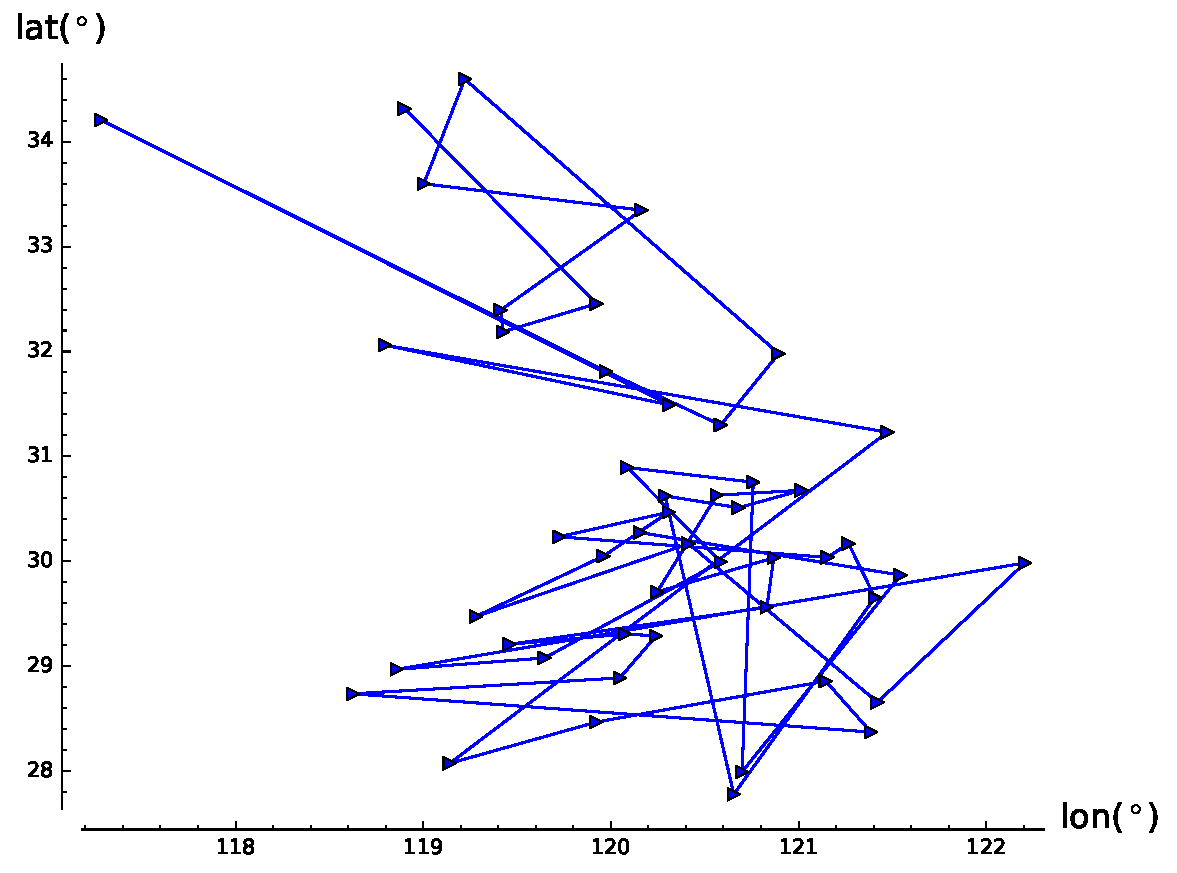
\includegraphics[width=.3\columnwidth]{init_map}} \quad  
	\subfloat[Transform into complete weight graph]{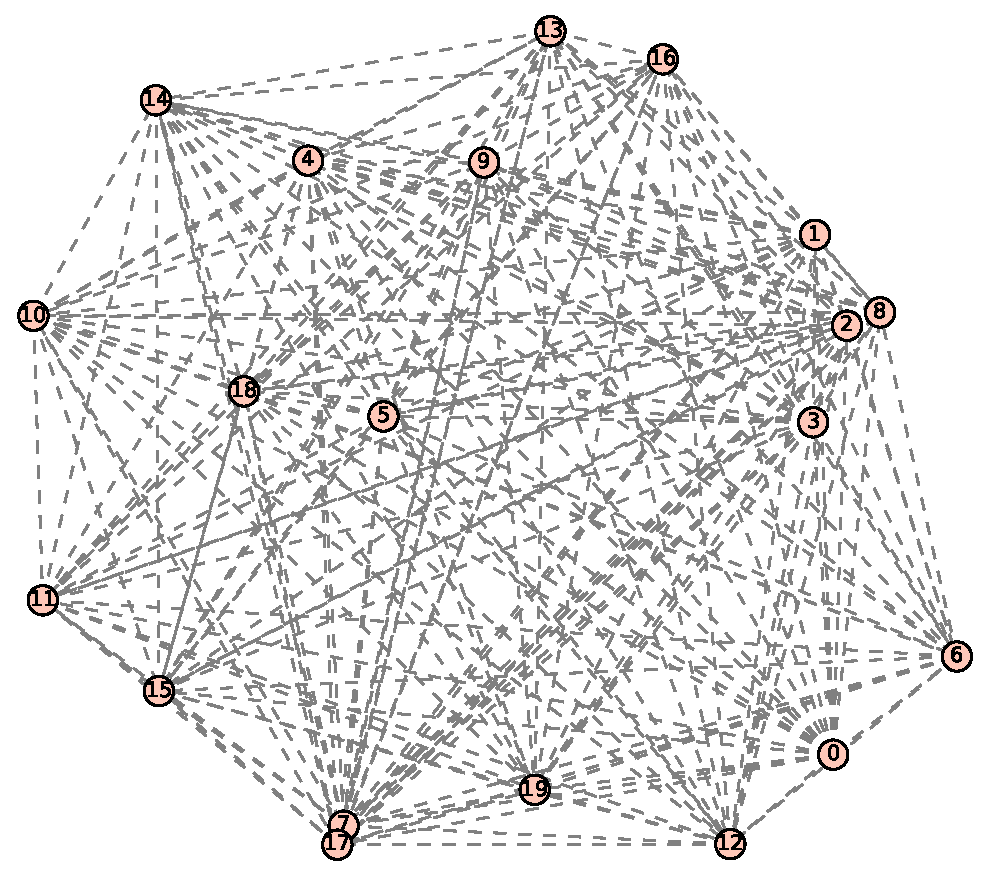
\includegraphics[width=.25\columnwidth]{topology}\label{fig:sage_top}}  \quad
	\subfloat[Plot according to locations]{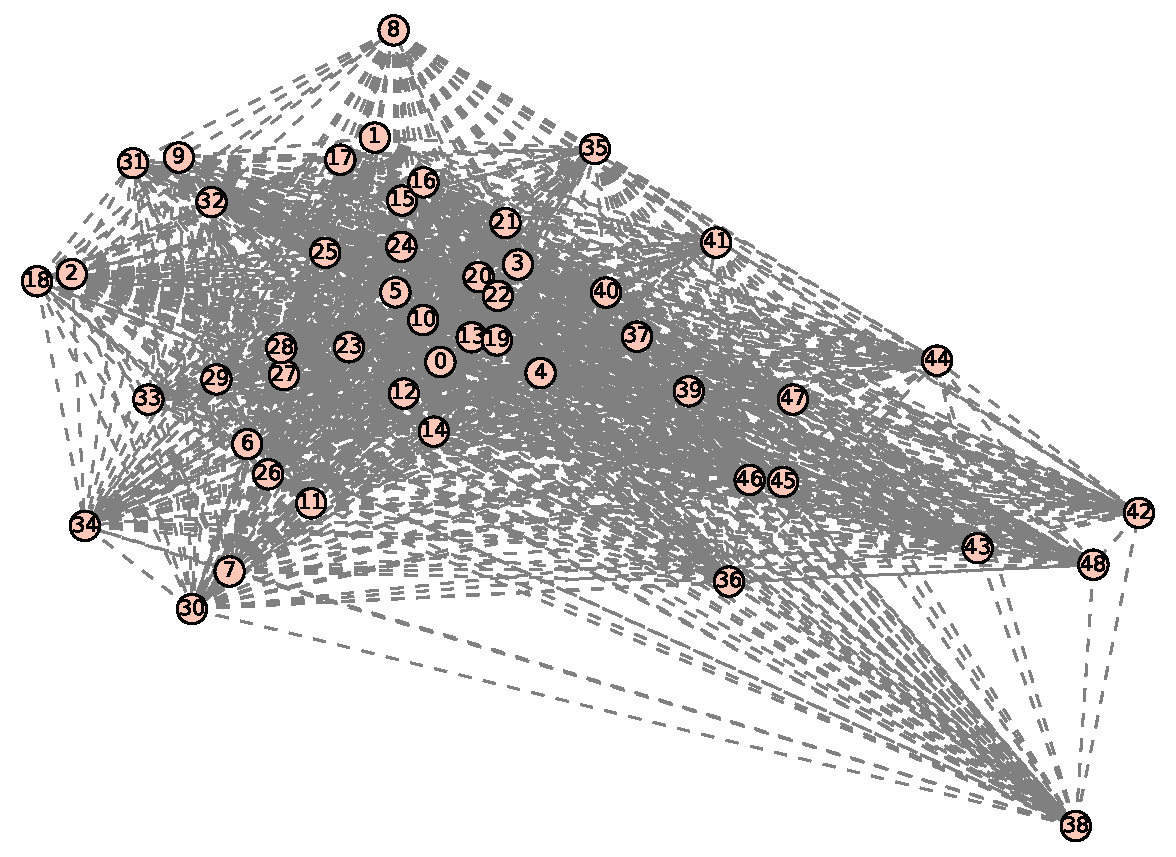
\includegraphics[width=.35\columnwidth]{trans_map}}
	\\
	\subfloat[The optimal solution find by ILP]{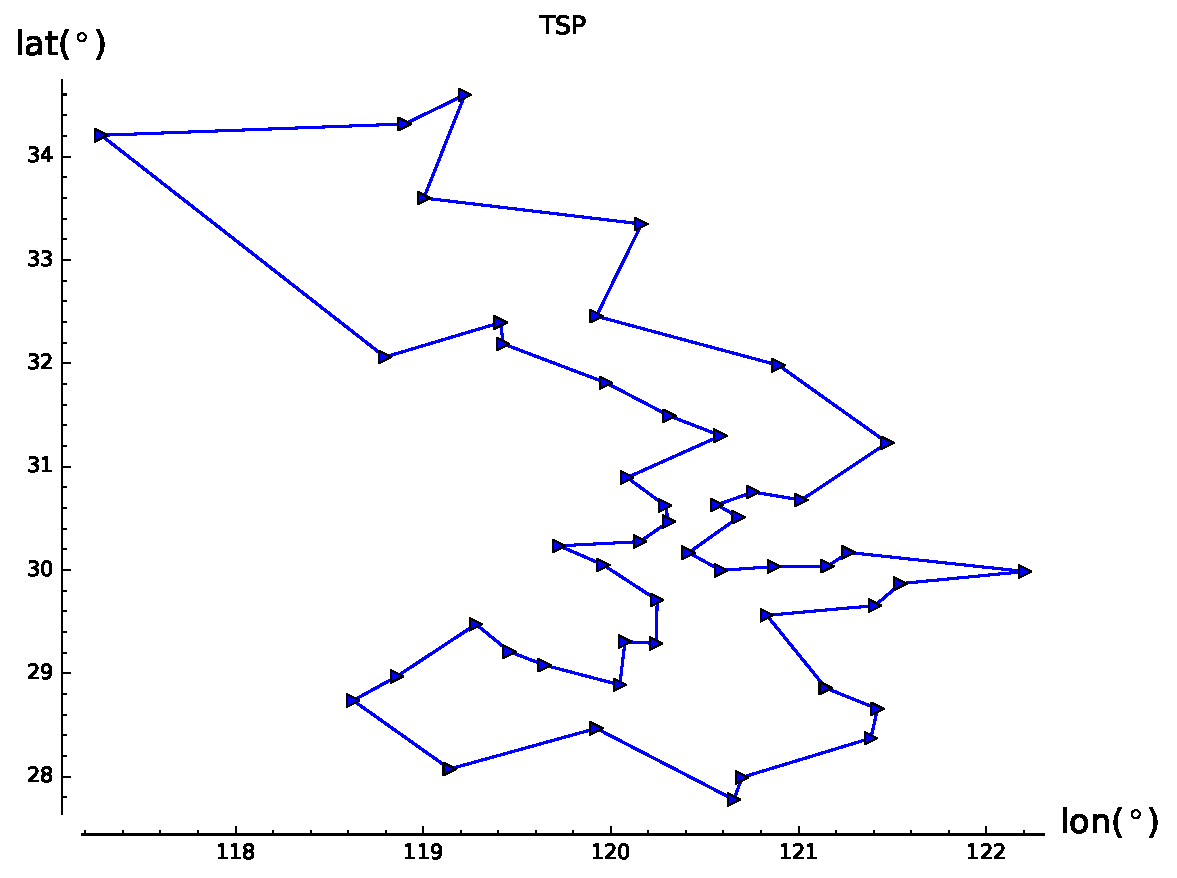
\includegraphics[width=.4\columnwidth]{tsp_res}\label{fig:tsp_res}}  \quad 
	\subfloat[The optimal solution find by Sage(also formulate problem as ILP to solve )]{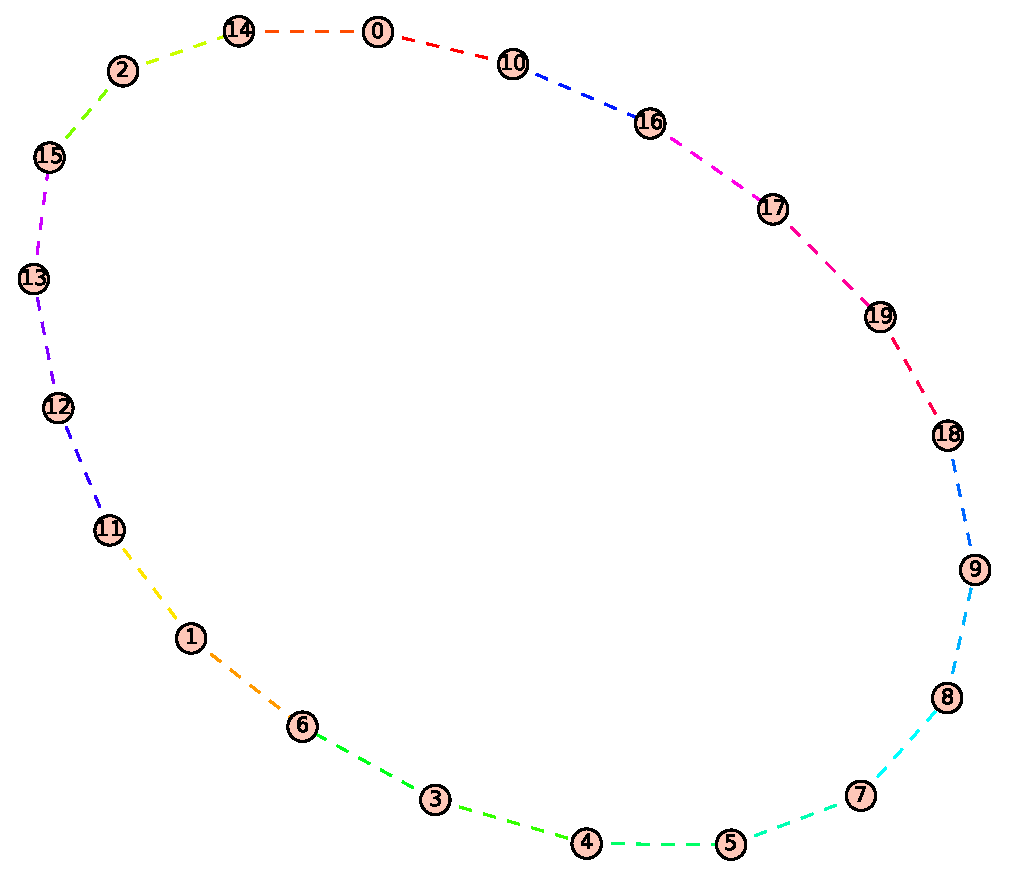
\includegraphics[width=.4\columnwidth]{tsp_sage} \label{fig:tsp_sage} }
	\caption[Results]{Fig~\vref{fig:tsp_res} is equivalent to Fig~\vref{fig:jiangzhehu} with correct (longitude, latitude) as coordinate. But when set the position information for Graph I use (latitude, longitude) mistakenly. We can see the solution find by \vref{code:sage2} is the same as Sage. In fact, I look into Sage's Source code, inspired by it and write new  formulation of symmetric TSP.} 
\end{figure}
\begin{figure}[H]
	\centering
	\subfloat[TSP on Hangzhou]{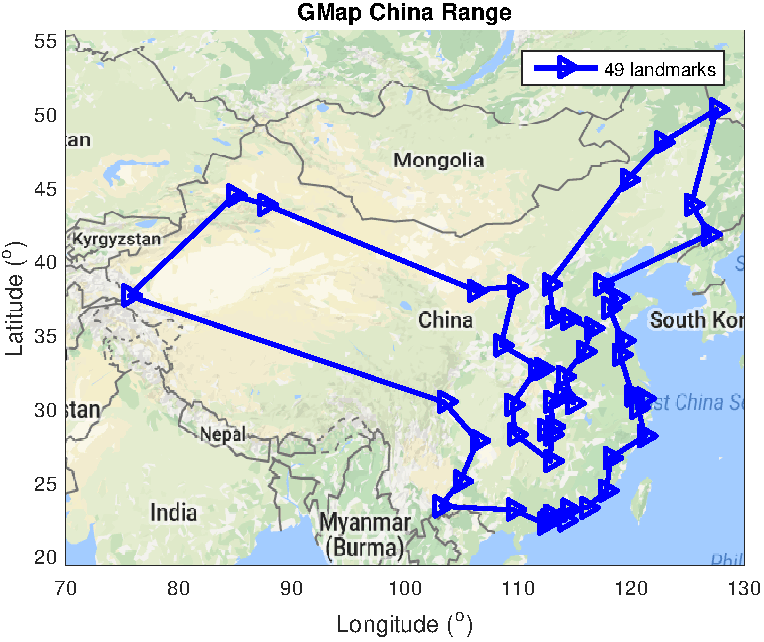
\includegraphics[width=.48\columnwidth]{GMap_Cn}} \   
	\subfloat[TSP on JiangZheHu]{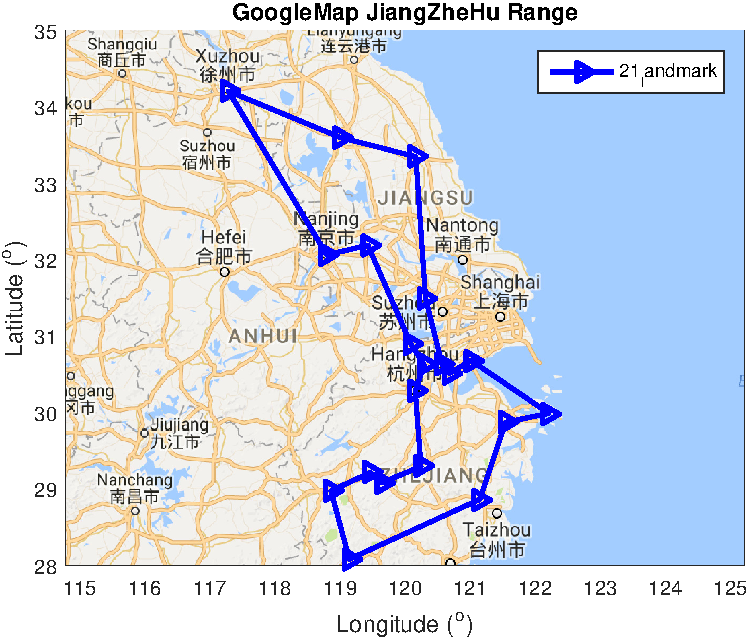
\includegraphics[width=.47\columnwidth]{GMap_Jzh}\label{fig:jiangzhehu}} 
	\caption[Results]{JiangZheHu is a wider range than Hangzhou. I am quite happy to solve a TSP on China range.} 
\end{figure}
\begin{figure}[H]
	\centering
	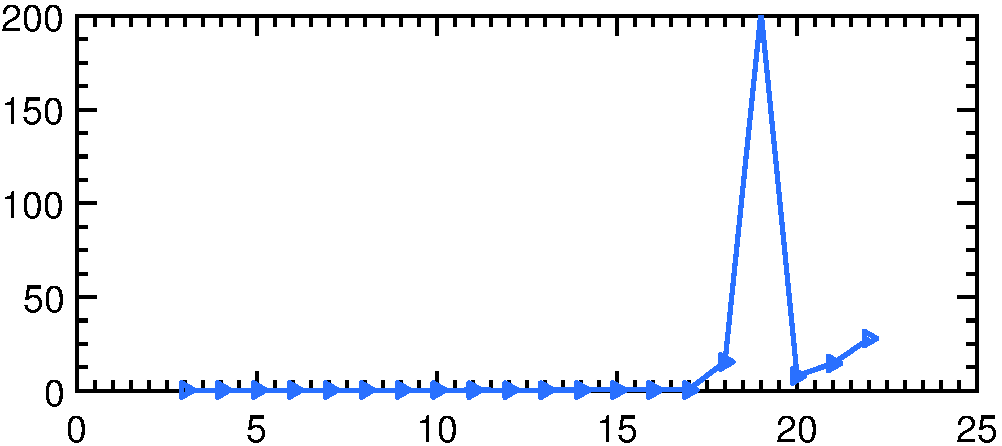
\includegraphics[width=.5\columnwidth]{benchmark}
	\caption[Running time]{X-axis: number of landmarks, Y-axis: elapsed time in seconds. For Asymmetric TSP, running time starts to grow explosively at $n=19$.  We can expect Symmetric TSP starts to grow explosively after $n=50$.}
	\label{fig:elaspe}.
\end{figure}
\section{Lab Code}
%My codes are somewhat lengthy, so I just put some important code, hope not to impact the compactness of this report. 
%I will clean and release the code on github later.
Here let me put some important code(the part for different ILP formulation of TSP ).
%	\subsubsection{Crawling Data of CHINA Landmarks}
%	\lstinputlisting[language=Python]{./code/test.py}
	\subsection{Symmetric Formulation} \label{code:sage}
	Here I use adjacent matrix. 
	\lstinputlisting[language=Python]{./code/sage.py}
	\subsection{Asymmetric Formulation}
	Here I use language of graph. 
	\lstinputlisting[language=Python]{./code/sage2.py} \label{code:sage2}
%	\subsubsection{Draw on GMap}
%	\lstinputlisting[language=Matlab]{./code/lOptHw.m}	
	%\textbf{\textcolor[rgb]{0.98,0.00,0.00}{Input matlab source:}}
	
	%some more text \textcolor[rgb]{0.98,0.00,0.00}{\textbf{Input C++ source:}}
	%\lstinputlisting[language=C++]{./code/mcmthesis-sudoku.cpp}
	
%			\section{Landmarks Around HangZhou }
%			\begin{longtable}{|l||l|l|} \hline
city & latitude & longitude \\ \hline \hline
$\text{\texttt{Hangzhou}}$ & $30.274085$ & $120.15507$ \\ \hline
$\text{\texttt{Ningbo}}$ & $29.868336$ & $121.54399$ \\ \hline
$\text{\texttt{Wenzhou}}$ & $27.993828$ & $120.699362$ \\ \hline
$\text{\texttt{Jiaxing}}$ & $30.753924$ & $120.758543$ \\ \hline
$\text{\texttt{Huzhou}}$ & $30.894348$ & $120.086823$ \\ \hline
$\text{\texttt{Shaoxing}}$ & $29.995762$ & $120.586109$ \\ \hline
$\text{\texttt{Jinhua}}$ & $29.079175$ & $119.647421$ \\ \hline
$\text{\texttt{Quzhou}}$ & $28.97008$ & $118.859457$ \\ \hline
$\text{\texttt{Zhoushan}}$ & $29.985295$ & $122.207216$ \\ \hline
$\text{\texttt{Taizhou}}$ & $28.65638$ & $121.42076$ \\ \hline
$\text{\texttt{Xiaoshan}}$ & $30.168016$ & $120.414929$ \\ \hline
$\text{\texttt{Jiande}}$ & $29.474871$ & $119.281164$ \\ \hline
$\text{\texttt{Fuyang}}$ & $30.048692$ & $119.960076$ \\ \hline
$\text{\texttt{Yongning{ }Rd}}$ & $30.4682595$ & $120.308662$ \\ \hline
$\text{\texttt{Lin'an}}$ & $30.233873$ & $119.724733$ \\ \hline
$\text{\texttt{Yuyao}}$ & $30.037192$ & $121.154634$ \\ \hline
$\text{\texttt{Cixi}}$ & $30.169665$ & $121.266579$ \\ \hline
$\text{\texttt{Fenghua}}$ & $29.655143$ & $121.406995$ \\ \hline
$\text{\texttt{Rui'an}}$ & $27.778657$ & $120.655148$ \\ \hline
$\text{\texttt{Deqing}}$ & $30.623883$ & $120.289015$ \\ \hline
$\text{\texttt{Haining}}$ & $30.510659$ & $120.680757$ \\ \hline
$\text{\texttt{Pinghu}}$ & $30.677233$ & $121.015142$ \\ \hline
$\text{\texttt{Tongxiang}}$ & $30.630173$ & $120.565099$ \\ \hline
$\text{\texttt{Zhuji}}$ & $29.708692$ & $120.246863$ \\ \hline
$\text{\texttt{Shangyu}}$ & $30.033121$ & $120.868122$ \\ \hline
$\text{\texttt{Shengzhou}}$ & $29.56141$ & $120.831026$ \\ \hline
$\text{\texttt{Lanxi}}$ & $29.208919$ & $119.460526$ \\ \hline
$\text{\texttt{Yiwu}}$ & $29.306757$ & $120.07514$ \\ \hline
$\text{\texttt{Dongyang}}$ & $29.289648$ & $120.241566$ \\ \hline
$\text{\texttt{Yongkang}}$ & $28.888555$ & $120.047651$ \\ \hline
$\text{\texttt{Jiangshan}}$ & $28.737223$ & $118.626974$ \\ \hline
$\text{\texttt{Wenling}}$ & $28.372506$ & $121.385604$ \\ \hline
$\text{\texttt{Linhai}}$ & $28.858457$ & $121.145046$ \\ \hline
$\text{\texttt{Lishui}}$ & $28.46763$ & $119.922796$ \\ \hline
$\text{\texttt{Longquan}}$ & $28.07465$ & $119.141474$ \\ \hline
$\text{\texttt{Shanghai}}$ & $31.230416$ & $121.473701$ \\ \hline
$\text{\texttt{Nanjing}}$ & $32.060255$ & $118.796877$ \\ \hline
$\text{\texttt{Wuxi}}$ & $31.49117$ & $120.31191$ \\ \hline
$\text{\texttt{Xuzhou}}$ & $34.205768$ & $117.284124$ \\ \hline
$\text{\texttt{Changzhou}}$ & $31.811226$ & $119.974062$ \\ \hline
$\text{\texttt{Suzhou}}$ & $31.298979$ & $120.58529$ \\ \hline
$\text{\texttt{Nantong}}$ & $31.980172$ & $120.894291$ \\ \hline
$\text{\texttt{Lianyungang}}$ & $34.596653$ & $119.221611$ \\ \hline
$\text{\texttt{9{ }Xueyuan{ }Rd}}$ & $33.598607$ & $119.0033924$ \\ \hline
$\text{\texttt{Yancheng}}$ & $33.347316$ & $120.16366$ \\ \hline
$\text{\texttt{Yangzhou}}$ & $32.394213$ & $119.412947$ \\ \hline
$\text{\texttt{Zhenjiang}}$ & $32.187849$ & $119.425836$ \\ \hline
$\text{\texttt{Taizhou}}$ & $32.455536$ & $119.922933$ \\ \hline
$\text{\texttt{745{ }Country{ }Rd}}$ & $34.3147372$ & $118.901079$ \\ \hline
\end{longtable}		
\end{appendices}


\begin{thebibliography}{99}
	\bibitem{bib:gmap} \url{http://www.openstreetmap.org/export#map=16/30.2802/120.1700}
	\bibitem{bib:github/sage/tsp} \url{https://github.com/sagemath/sagelib/blob/master/sage/graphs/generic_graph.py}	
	\bibitem{bib:wiki}  \url{https://en.wikipedia.org/wiki/Haversine_formula}
	\bibitem{bib:wiki/tsp} \url{https://en.wikipedia.org/wiki/Travelling_salesman_problem#Solving_by_conversion_to_symmetric_TSP}
\end{thebibliography}

\end{document}